\chapter*{Introducción}
\addcontentsline{toc}{chapter}{Introducción}

% La introducción no cuenta como primer capítulo
\section{Motivación y contexto}
\noindent La siniestralidad vial en la Ciudad de México constituye un problema de salud pública de primer orden. Entre 2014 y 2023 la ciudad registró, en promedio, 85,150 accidentes viales anuales, con un saldo de 37,638 personas lesionadas y 383 defunciones al año, es decir, más de una muerte diaria solo en el lugar del incidente. Estas cifras, provenientes de los registros del Centro de Comando, Control, Cómputo, Comunicaciones y Contacto Ciudadano (C5), ilustran la magnitud del problema y sus implicaciones tanto para la seguridad vial como para el sistema de salud.\\
% aquí debe ir la sección que explica que el gobierno se ha dado cuenta del problema

% una vez que ya explicamos que el gobierno está conciente de que hay accidentes y que la velocidad es un problema entra la parte de las fotocívicas y de las fotomultas.
\indent Más allá del nivel absoluto de incidentes, la evolución reciente de estos eventos sugiere que la situación se ha vuelto especialmente preocupante en los últimos años. La Figura 1 muestra la trayectoria del número total de accidentes viales entre 2014 y 2023, desagregados en accidentes menores, con lesionados y fatales. El sistema de fotocívicas entró en vigor el 22 de abril de 2019. Hasta ese momento se observaba una tendencia a la baja tanto en el número total de incidentes como en los accidentes fatales anuales. Sin embargo, tras una caída pronunciada en 2020 ---muy probablemente asociada a la reducción de la movilidad durante la pandemia de COVID‑19--- se registra un repunte en el número de incidentes viales, especialmente en los de mayor severidad.

\begin{figure}
    \centering
    \caption{Número anual de incidentes viales en la CDMX}
    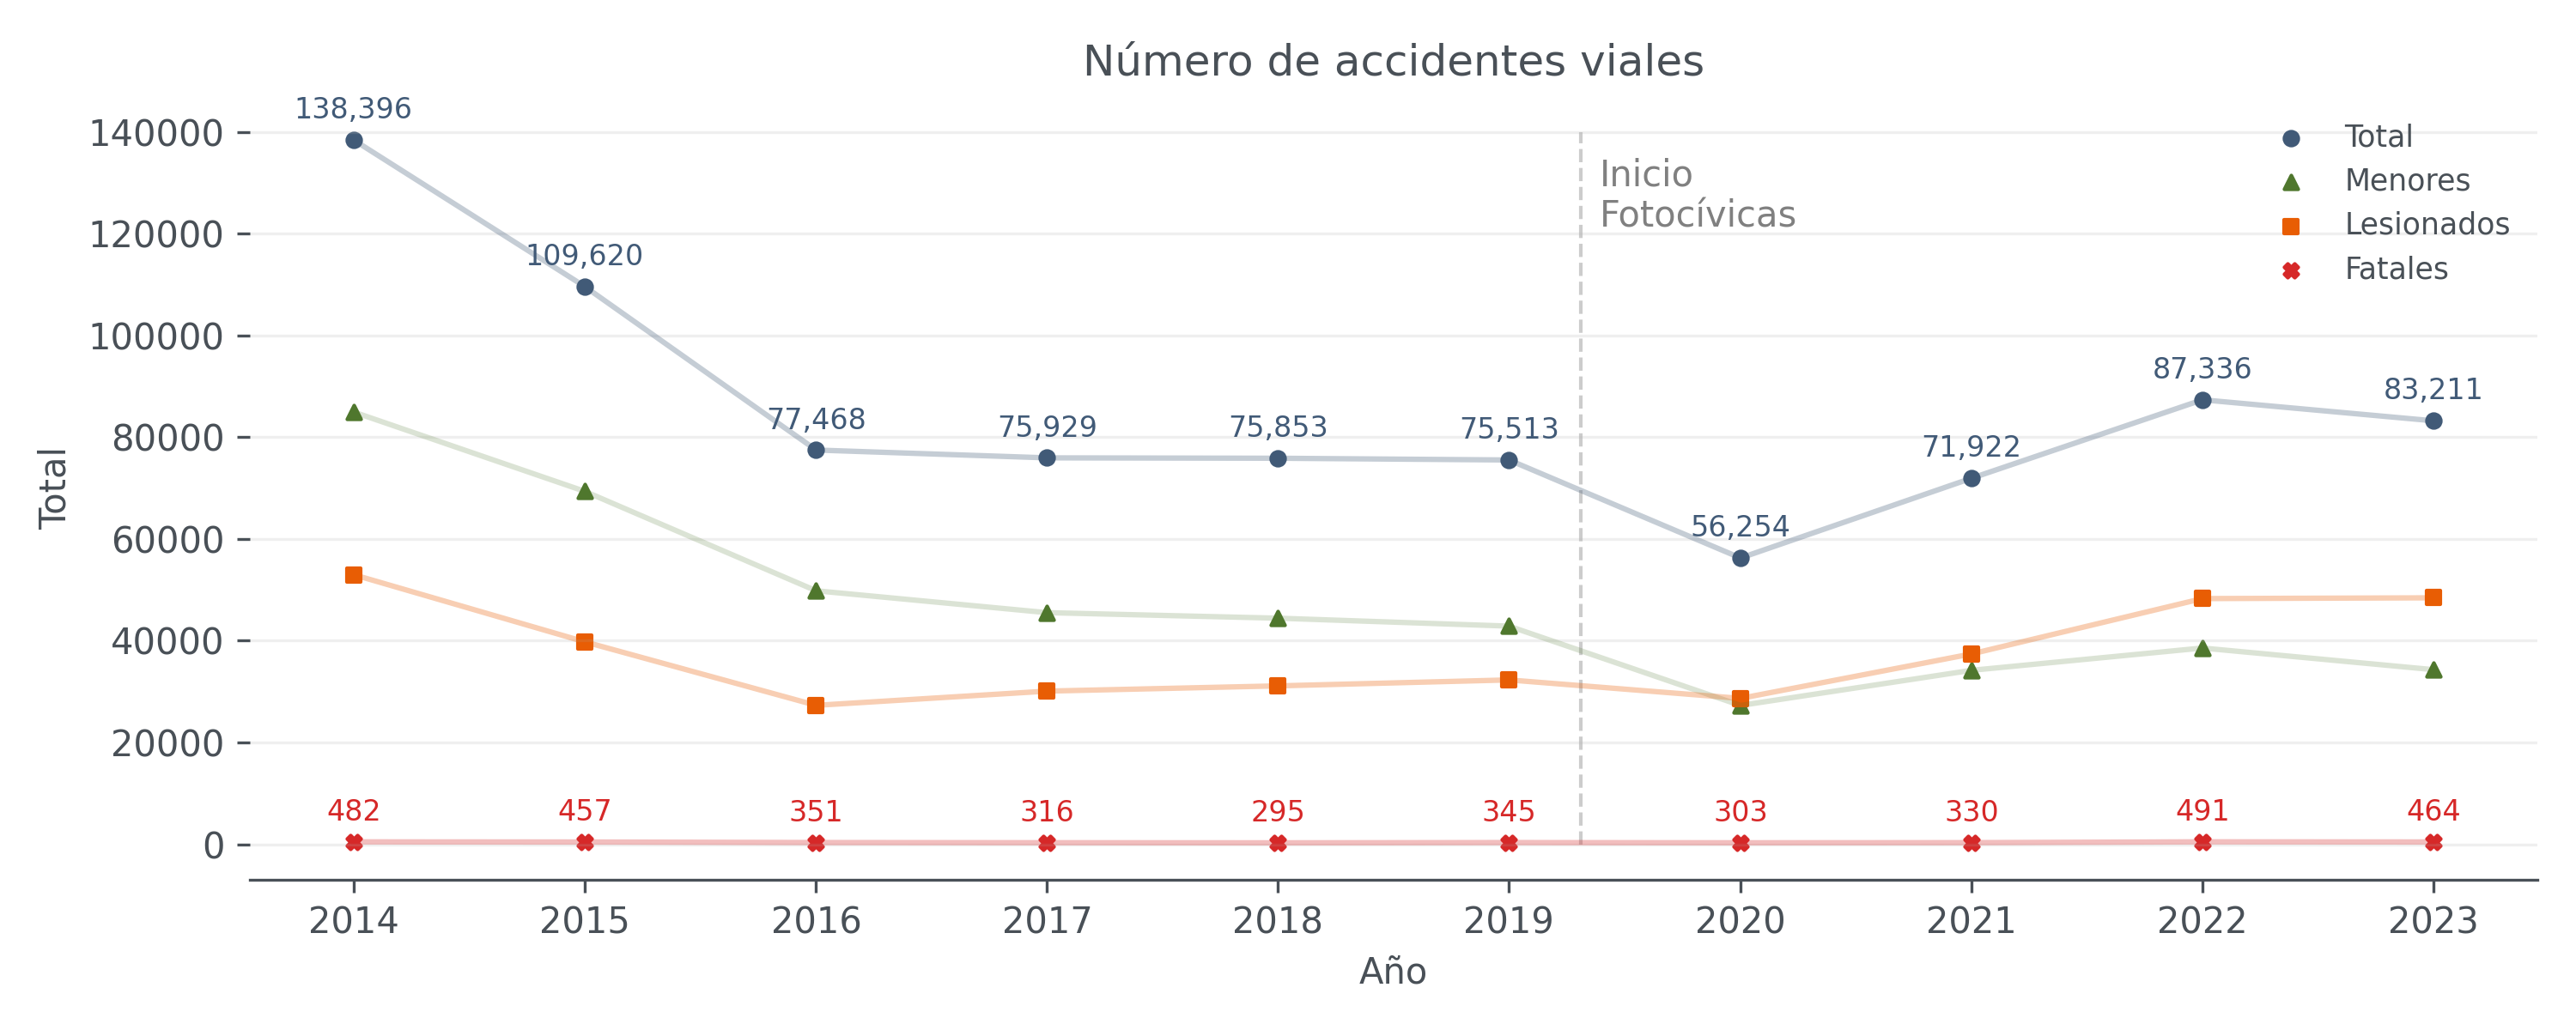
\includegraphics[width=1\linewidth]{Imagenes/yearly-number-of-incidents.png}
    \label{fig:placeholder}
\end{figure}

Este cambio de tendencia se aprecia con claridad al comparar 2018, último año completo previo a la implementación de las fotocívicas, con 2023. En ese periodo, los incidentes totales pasaron de 75,853 a 83,211, lo que implica un aumento de 9.7\%. Más grave aún, los accidentes con al menos una persona fallecida se incrementaron de 295 a 464, es decir, un aumento del 57\%. La Figura 2, que presenta únicamente el número de accidentes fatales por año, muestra un mínimo en 2018 seguido de un crecimiento sostenido. Aunque con esta evidencia descriptiva no es posible atribuir causalmente estos cambios a un solo factor, sí resulta claro que la introducción del programa de fotocívicas no evitó el repunte observado en los accidentes más graves en el total agregado de la ciudad.

\begin{figure}
    \centering
    \caption{Número anual de accidentes fatales}
    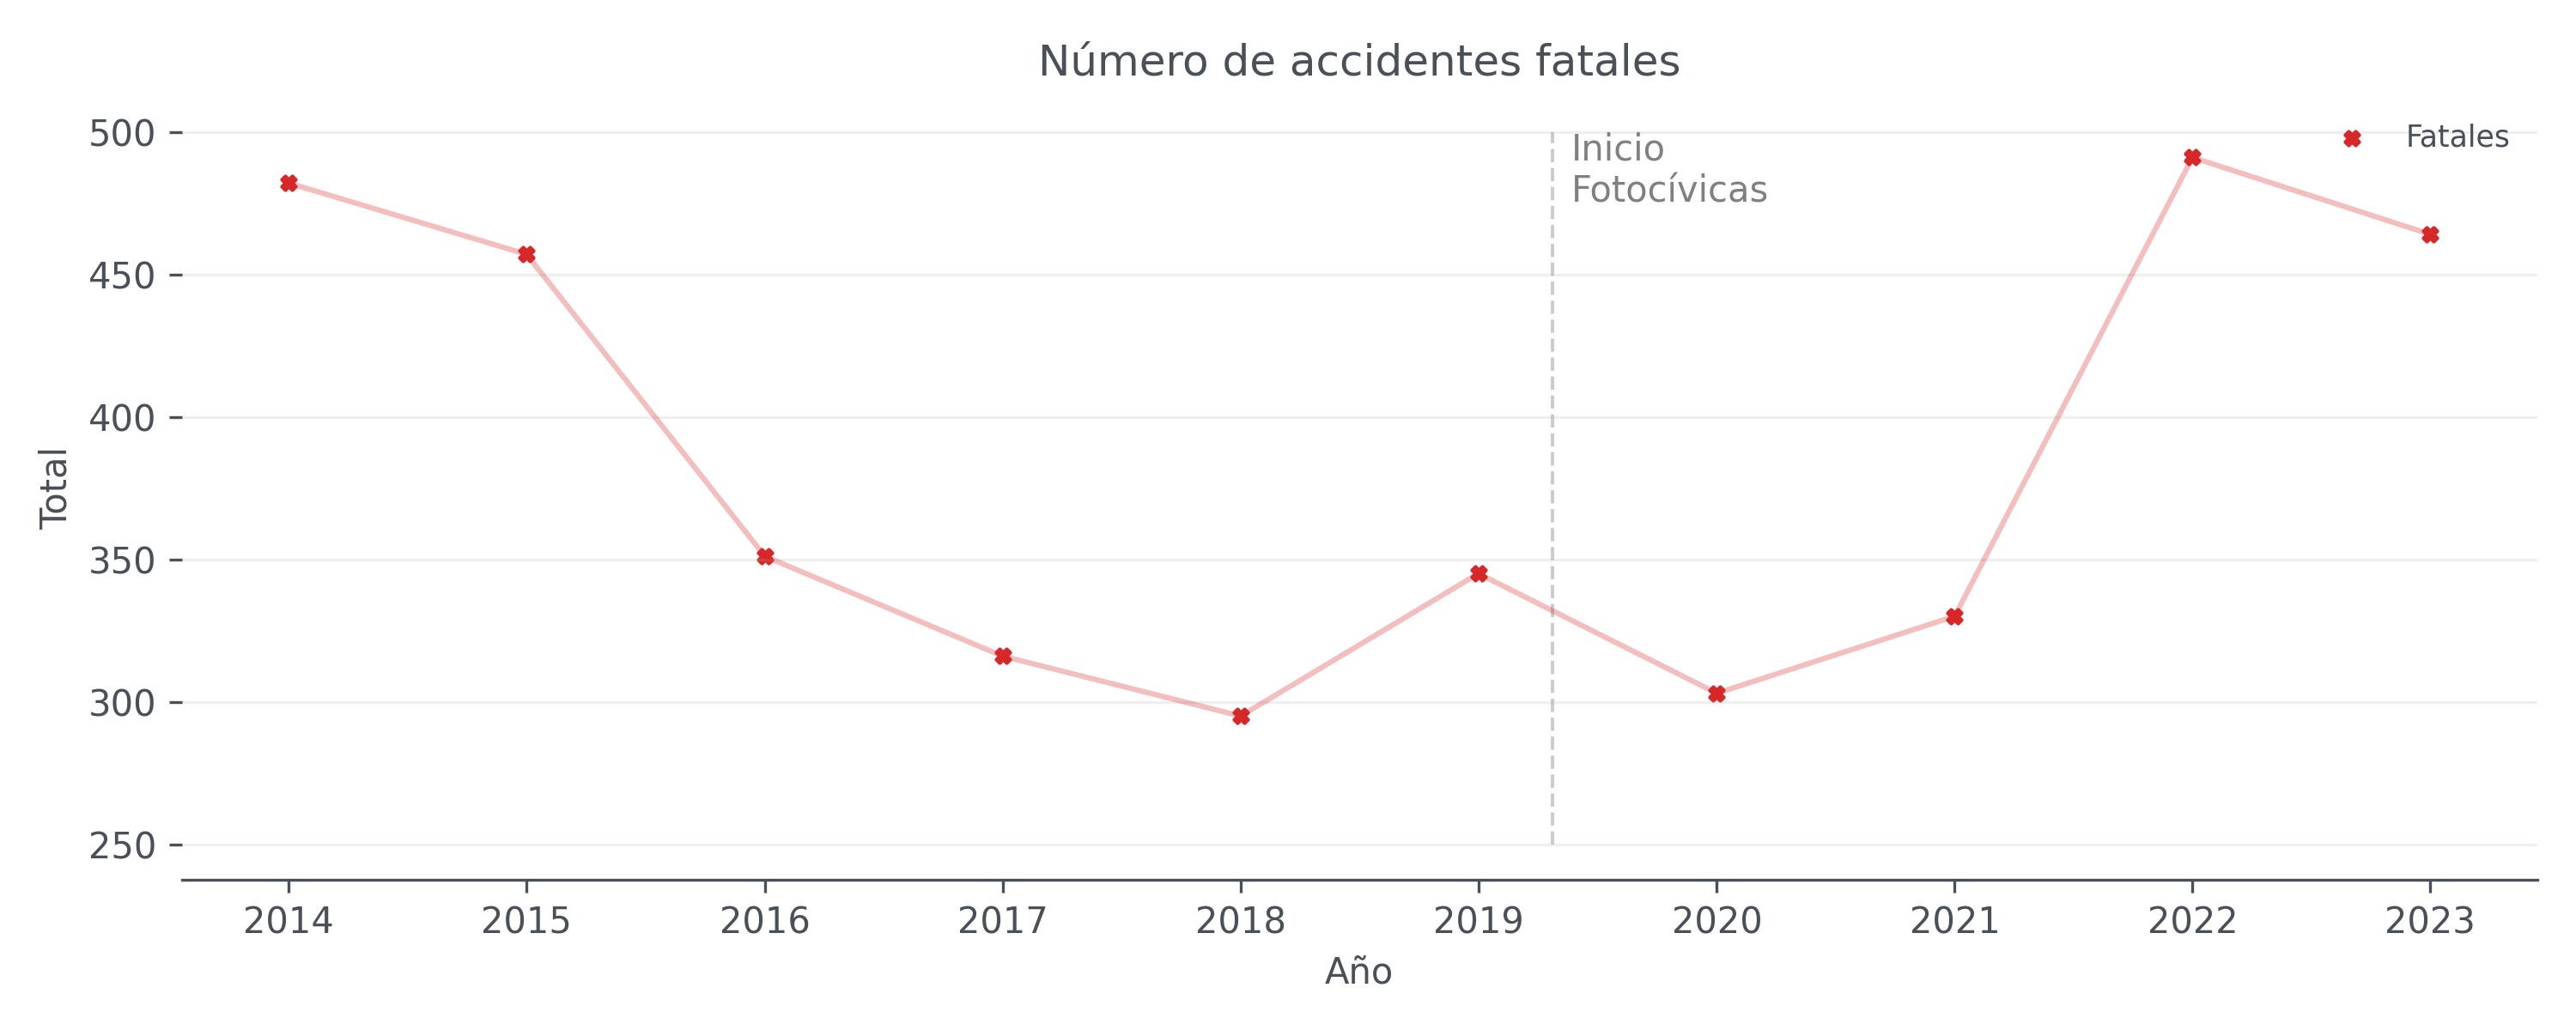
\includegraphics[width=1\linewidth]{Imagenes/yearly-fatal-number-of-incidents}
    \label{fig:figure-here}
\end{figure}

La composición de los siniestros también se ha modificado. Como se observa en la Figura 1, la disminución de 2020 en el número total de incidentes se explica principalmente por la reducción de los accidentes menores, mientras que los accidentes con lesionados o fallecidos no se reducen en la misma proporción. A partir de 2020, los incidentes con personas lesionadas superan a los accidentes considerados menores y se mantienen por encima hasta 2023, ampliando cada año la brecha entre ambos tipos de eventos. Es decir, no solo sigue habiendo muchos accidentes, sino que una fracción creciente de ellos tiene consecuencias más severas.\\

Este diagnóstico coincide con lo reportado por la Secretaría de Movilidad (SEMOVI) en el Programa Integral de Seguridad Vial de la Ciudad de México 2021–2024, donde se documenta que la reducción en la afluencia vehicular durante la pandemia ---aproximadamente del 45\%--- permitió mayores velocidades de circulación y que el aumento relativo de incidentes con lesionados y fallecidos se concentró en vías primarias y de acceso controlado. En otras palabras, el propio gobierno local reconoce que la velocidad y las características de la infraestructura vial juegan un papel central en la siniestralidad reciente.\\ 

Para analizar este fenómeno y evaluar la efectividad de las intervenciones de control de velocidad es necesario contar con información adecuada sobre los incidentes viales. Existen diversas fuentes de datos que ofrecen perspectivas complementarias. Por un lado, la Secretaría de Seguridad Ciudadana (SSC) publica registros georreferenciados de hechos de tránsito a partir de junio de 2018, pero estos datos solo incluyen incidentes con personas lesionadas y cubren un periodo relativamente corto en relación con la entrada en vigor del sistema de fotocívicas, lo que dificulta construir una ventana simétrica de al menos tres años antes y después de la política.\\

Por otro lado, los datos del C5 ofrecen una cobertura temporal más amplia y un panorama más completo de la siniestralidad. Esta base integra reportes de llamadas al 911, incidentes detectados por las cámaras de videovigilancia y registros levantados por las autoridades en el lugar de los hechos. Además, incluye tanto accidentes con lesionados y fallecidos como incidentes menores, que de otra forma quedarían subrepresentados. Por estas razones, en esta tesis empleo los registros del C5 como fuente principal para el análisis.\\ 

\section{Programas de control de velocidad en la Ciudad de México}
\noindent El control de la velocidad ha adquirido relevancia mundial como estrategia central para mejorar la seguridad vial. La Guía para el Control de la Velocidad (Secretaría de Salud, 2018) identifica la velocidad como el principal factor de riesgo en la ocurrencia y severidad de los siniestros viales y destaca que “el 90\% de los automovilistas se considera un conductor por encima del promedio y de bajo riesgo”. Esta sobreconfianza convive con una infraestructura pensada para favorecer traslados rápidos y con una cultura que valora la velocidad por encima de la seguridad. La misma guía documenta que la probabilidad de sobrevivir a un atropellamiento se reduce de 90\% a 30 km/h a solo 17\% a 50 km/h, lo que refuerza la necesidad de limitar las velocidades efectivas en la red vial.\\

\indent En la Ciudad de México, la principal herramienta de control automatizado de la velocidad han sido los programas de fotomultas y, posteriormente, de fotocívicas. El Programa Fotomultas comenzó a operar en diciembre de 2015 con un diseño claramente recaudatorio: el exceso de velocidad detectado por los radares se traducía en sanciones económicas aplicadas al propietario del vehículo. Este esquema fue objeto de críticas por su orientación a la recaudación y por la falta de transparencia en la operación.\\

En abril de 2019 el gobierno de la ciudad sustituyó el esquema de fotomultas por el sistema de fotocívicas, con el argumento de transitar de una política centrada en la recaudación hacia una enfocada en el cambio de conducta. El nuevo modelo se basa en un sistema de puntos asociado a las placas de los vehículos registrados en la ciudad: cada placa inicia con diez puntos y, por cada infracción detectada, se pierde un punto (cinco puntos si el límite de velocidad se excede en más de 40\%). La forma de resarcir estas infracciones ya no es el pago de una multa, sino la realización de cursos educativos y trabajo comunitario. Cuando una placa pierde más de dos puntos, su propietario no puede verificar el vehículo hasta cumplir con las sanciones correspondientes (no es posible circular si el vehículo no está verificado). Para los vehículos con placas foráneas, en cambio, el esquema mantiene las sanciones económicas.\\

La implementación de fotocívicas vino acompañada de una reubicación de los radares. De acuerdo con la SEMOVI, las cámaras se reubicaron hacia tramos con mayor incidencia de hechos de tránsito, en particular aquellos con más muertos y lesionados, así como en puntos con elevados volúmenes de tránsito y donde el límite de velocidad tendía a no respetarse. En total se instalaron 138 dispositivos, de los cuales 58 provenían del sistema anterior y 80 fueron nuevos. Aunque la lógica oficial no menciona explícitamente indicadores como el exceso medio de velocidad, sí enfatiza la concentración de incidentes y la importancia de las vías primarias y de acceso controlado como criterio de ubicación.\\

En la práctica, sin embargo, el nuevo sistema ha seguido funcionando en gran medida como un esquema de sanciones económicas. Los registros de la propia autoridad, como lo podemos observar en la Figura 3, muestran que la proporción de sanciones cívicas ha oscilado entre 14\% y 24\% del total, lo que implica que la mayoría de las infracciones se ha traducido en multas monetarias. Esto puede deberse, entre otras razones, al elevado número de vehículos con placas foráneas que circulan por la ciudad o a que los propietarios con placas locales internalizan mejor el riesgo de sanción y ajustan su comportamiento. Aunque el análisis detallado de estas causas excede el alcance de esta tesis, el dato es relevante porque sugiere que la experiencia de los conductores con el sistema se asemeja más a un esquema de multas que al modelo cívico originalmente planteado.\\

\begin{figure}
    \centering
    \caption{Total de infracciones por tipo de sanción}
    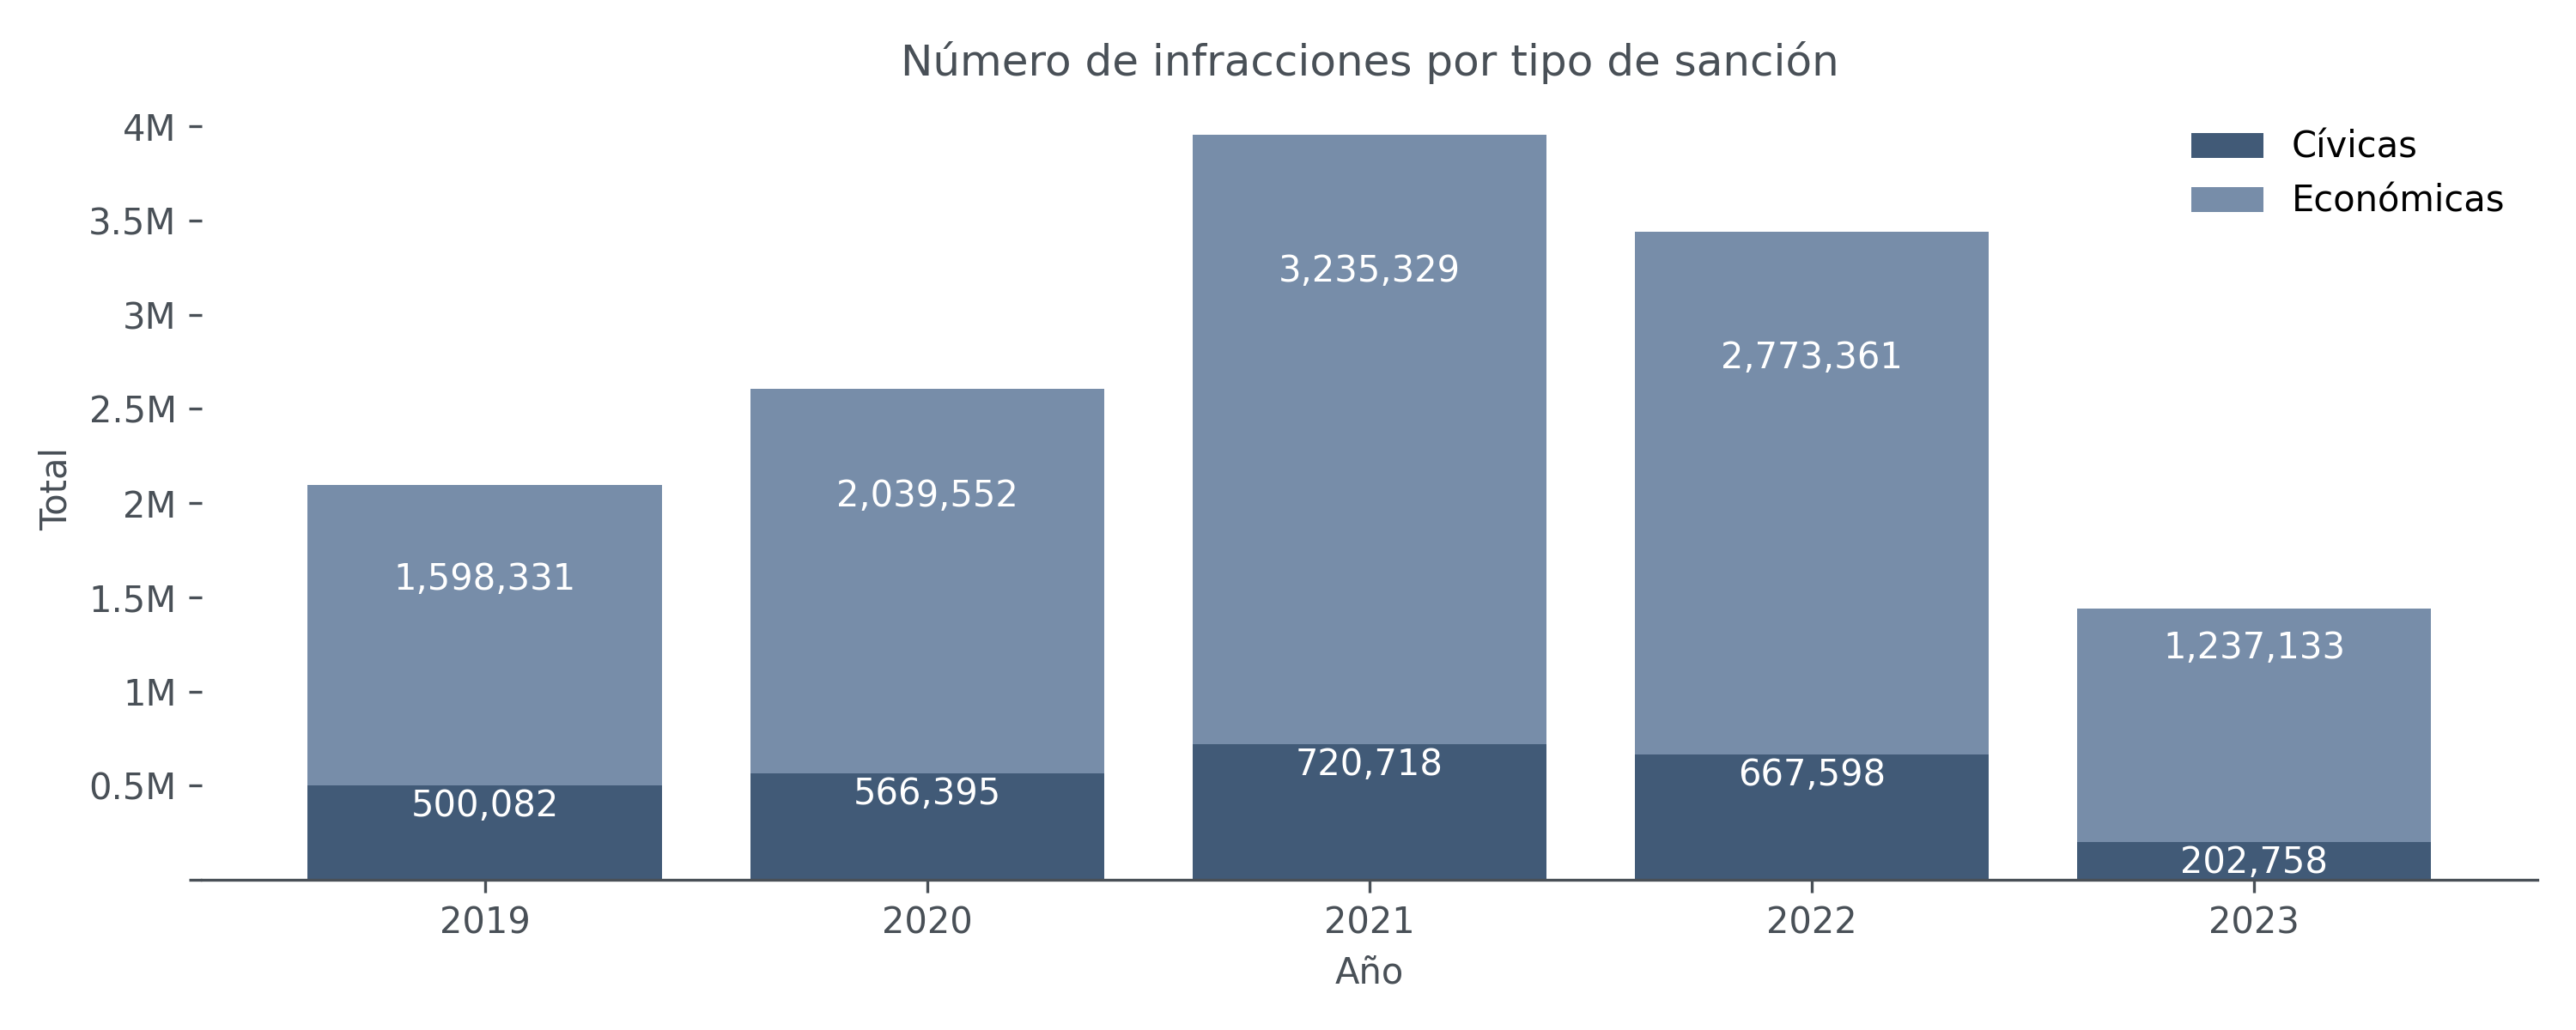
\includegraphics[width=1\linewidth]{Imagenes/yearly-number-of-sanctions.png}
\end{figure}

\section{Pregunta de investigación e hipótesis}
\noindent En este contexto, es natural preguntarse si las cámaras de velocidad realmente han tenido el efecto que prometían sobre la seguridad vial de la ciudad. A primera vista, podría pensarse que, al menos en los puntos donde se instalaron, deberían observarse menos incidentes, en particular menos hechos con personas lesionadas o fallecidas. Sin embargo, las tendencias mostradas en las figuras anteriores, así como el repunte reciente de los accidentes fatales, hacen que esta intuición deje de ser tan obvia. La pregunta que guía esta tesis es precisamente esa: \textbf{¿qué tanto han cambiado los incidentes viales en torno a las cámaras de velocidad desde la implementación del sistema de fotocívicas?}\\

En esta tesis parto de la hipótesis de que las cámaras de velocidad del sistema de fotocívicas reducen el número de incidentes viales en su entorno, con un efecto relativamente mayor en los siniestros más graves (con lesionados y, sobre todo, con fallecidos), en magnitudes similares a las reportadas en la literatura internacional (del orden de 10–20\%). Para poner a prueba esta hipótesis utilizo los registros del C5 y construyo unidades de análisis espaciales. Primero ensayo un enfoque basado en una malla de cuadrículas sobre toda la ciudad, pero encuentro que los resultados son muy sensibles a cambios mínimos en el diseño del grid, lo que revela problemas de robustez y me lleva a descartar este esquema.\\

A partir de ello adopto un segundo método, inspirado en trabajos como Li et al. (2020), que define áreas circulares alrededor de cada cámara. Construyo para cada una un grupo de control mediante Propensity Score Matching, usando como covariables la siniestralidad previa, características de la infraestructura vial y proxies de movilidad basados en afluencia al metro y radares de conteo de tránsito vehicular. Para estimar los efectos utilizo un método de Diferencia en Diferencias, evaluando la interacción del tiempo con el tratamiento en mis unidades tratadas contra las de control.\\

En términos generales, los resultados muestran que no existe evidencia estadística suficiente para afirmar que las cámaras generaron una reducción localizada de la siniestralidad en su entorno inmediato. Al mismo tiempo, sí se observa una caída agregada de los incidentes en áreas tratadas y de control después de la implementación del programa, lo que sugiere que la evidencia previa para la ciudad puede estar captando cambios sistémicos más que efectos causales estrictamente locales alrededor de los radares.

\section{Contribuciones a la literatura}
\noindent Solo es posible entender la justificación de esta tesis bajo el contexto de la literatura existente en la Ciudad de México, pues no es el primer estudio que analiza el efecto de las cámaras de velocidad en la siniestralidad vial. Bajo este supuesto, es más fácil ver cómo encaja precisamente ahí donde hay oportunidades de traer lo que la literatura internacional ha encontrado al contexto de la Ciudad de México. 

En primer lugar, se busca identificar efectos locales alrededor de las cámaras de velocidad, lo cual se logra creando áreas circulares de distintos radios concéntricos en cada uno de los radares, dando como resultado no solo una imagen estática de lo que ocurre a una distancia determinada, sino que permite tener una historia más clara de lo que ocurre conforme nos vamos alejando de los radares. 

En segundo lugar, se busca construir un grupo de control que pueda representar de manera más fiel un contrafactual de lo que realmente hubiera ocurrido de no haberse instalado los radares, para lo cual se hace uso del \textit{Propensity Score Matching}, calculando la probablidad de recibir tratamiento con base en variables que representan la siniestralidad histórica de cada área, atributos de la infraestructura vial y medidas de exposición, como lo son la afluencia diaria en estaciones de metro cercanas a cada área. 

Se busca además controlar de forma explícita por los cambios en movilidad asociados a la pandemia por Covid-19, usando datos de las estaciones de conteo permanentes de la SICT, algo que había sido omitido en estudios anteriores. 

Por último, este análisis permite distinguir entre cambios agregados en la siniestralidad y efectos que son directamente atribuibles a las cámaras de velocidad, lo que ayuda a entender por qué estudios previos han llegado a conclusiones distintas respecto al programa de Fotocívicas en la CDMX.